% =====================================================================
% ICLR 2027 submission -- SRQ
%
% BUILD NOTES (read before compiling):
%   1. Download https://media.iclr.cc/Conferences/ICLR2027/iclr-2027-style-files.zip
%      and place iclr2027_conference.sty / .bst next to this file.
%      The \usepackage line below assumes the usual ICLR naming; adjust if
%      the 2027 pack renames it.
%   2. Bibliography: references_iclr2027.bib
%   3. HARD LIMITS: 9 pages main text (10 for the rebuttal revision).
%      References and appendix do NOT count. Overlength = desk reject.
%   4. Submission is double-blind. Do not add author names until acceptance.
%
% PAGE BUDGET (target, keep this in sync while editing):
%   p1   Intro + Fig 1
%   p2   Related Work (4 groups)
%   p3   Method: setup / square-root update / mixed precision
%   p4   Analysis: recurrence, ridge bound, margin certificate
%   p5   5.1 fixed precision does not scale + 5.2 why  (Fig 2, Fig 3)
%   p6   5.3 resolution: budget-locked allocation      (Table 1)
%   p7   5.4 factor structure + 5.5 portability        (Table 2, 3)
%   p8   5.6 equal-budget + memory + Limitations       (Fig 4)
%   p9   Conclusion + Reproducibility + AI use statement
% =====================================================================

\documentclass{article}
\usepackage{iclr2027_conference,times}

\usepackage{amsmath,amssymb,amsthm}
\usepackage{booktabs}
\usepackage{multirow}
\usepackage{graphicx}
\usepackage{microtype}
\usepackage{hyperref}
\usepackage{url}

\newtheorem{lemma}{Lemma}
\newtheorem{proposition}{Proposition}

\title{Error Accumulation Limits the Compression\\of Analytic Continual Learners}

% ---------------------------------------------------------------------
% DOUBLE BLIND: iclr2027_conference.sty replaces this whole block with
% "Anonymous authors / Paper under double-blind review" for as long as
% \iclrfinalcopy stays commented out. So put the REAL author details here
% -- they are hidden automatically and must NOT be deleted or faked.
% Uncomment \iclrfinalcopy only for the camera-ready version.
% ---------------------------------------------------------------------
% \iclrfinalcopy
\author{First Author, Second Author \\
Department \\
Institution \\
City, Country \\
\texttt{\{first,second\}@example.edu}}

\begin{document}
\maketitle

% =====================================================================
\begin{abstract}
Analytic continual learners replace stored exemplars with additive ridge
sufficient statistics, but the resulting Gram matrix dominates memory: at a
code width of $10{,}000$ it occupies 400\,MB in FP32. Compressing it is not a
direct application of optimizer-state quantization. Optimizer preconditioners
are exponential moving averages and therefore forget, whereas analytic
sufficient statistics accumulate monotonically, so quantization error never
decays. We show that this accumulation, rather than per-task reconstruction
fidelity, is what limits how far such state can be compressed.
Storing the regularized system as
a mixed-precision upper-triangular factor---FP32 diagonal, groupwise-INT8
strict upper triangle, blocked-QR updates---keeps the reconstructed system
positive definite by construction and reduces persistent learner state by
$76.7$--$78.1\%$ while changing average incremental accuracy (AIA) by at most
$0.083$ points across three datasets. Fixed INT8 precision nevertheless fails
to scale: from width $10{,}000$ to $20{,}000$ the local factor error grows by
only $1.6\%$ while classifier and logit error grow by $79\%$ and $100\%$, and
a preregistered accuracy-retention bound is violated. An exact perturbation
recurrence for the effective system predicts this behaviour, and a
budget-locked precision allocation that spends a fixed $25\%$ byte allowance
recovers Exact accuracy to within $0.005$ AIA points. Across FLY-CL, RanPAC
and GACL-style frontends, two frozen backbones and four datasets, every
comparison uses preregistered gates, train-only selection, and released
artifact hashes.
\end{abstract}

% =====================================================================
\section{Introduction}
\label{sec:intro}

Class-incremental learning requires a single predictor over all classes seen so
far, without task identity at inference. Replay methods preserve past knowledge
by retaining images, embeddings, or codes, so memory grows with the stream.
Analytic continual learners take the opposite route: they maintain sufficient
statistics of a closed-form ridge problem and never store a past sample
\citep{zhuang2022acil,zhuang2024foal}.

Removing replay does not remove state memory. Methods in this family expand a
frozen backbone feature into a high-dimensional code and accumulate a Gram
matrix over that code. FLY-CL \citep{zou2026flycl} uses a fly-inspired sparse
projection with winner-take-all (WTA) sparsification; RanPAC
\citep{mcdonnell2023ranpac} uses a random projection with ReLU. In both cases
the dominant persistent tensor is an $m\times m$ Gram matrix: at $m=10{,}000$,
that is $10^8$ FP32 entries, or 400\,MB---far larger than the classifier it
produces. Reducing $m$ shrinks the state but weakens the expanded
representation, and quantizing the Gram matrix directly can destroy positive
definiteness and make the ridge solve fail outright.

\paragraph{Why this is not optimizer-state quantization.}
A natural response is to import the factor-space quantization pattern
developed for second-order optimizers, where Cholesky factors of Shampoo
preconditioners are stored in 4 bits \citep{li2025fourbit,wang2024fourbitshampoo}.
We argue that the transfer is structurally incomplete. An optimizer
preconditioner is an exponential moving average: old contributions decay, so a
quantization error injected at step $t$ is geometrically forgotten. An analytic
continual learner accumulates
$A_t=\lambda I+\sum_{k\le t}\Phi_k^{\top}\Phi_k$ monotonically and never
forgets. Every re-encoding of the stored state therefore leaves a residue that
persists for the remainder of the stream. The relevant question is not how
accurately a single matrix can be quantized, but how the induced error in the
\emph{effective system} compounds over a task sequence---and what that implies
for the classifier that is solved from it.

\paragraph{Contributions.}
\begin{itemize}
\item[\textbf{C1}] \textbf{Finding.} We show that quantization error in
accumulating analytic state compounds across tasks, and that this---not local
reconstruction fidelity---is the binding constraint. At width $20{,}000$ the
local factor error is $1.6\%$ larger than at $10{,}000$, yet the resulting
classifier and logit errors are $79\%$ and $100\%$ larger, and a preregistered
$0.25$-point accuracy-retention bound fails. A same-byte control that
explicitly lowers local reconstruction error still misses the same bound,
confirming that local fidelity is the wrong target.

\item[\textbf{C2}] \textbf{Analysis.} We give an exact recurrence
$\Delta_t=\Delta_{t-1}+D_t$ for the effective-system error, a spectral
accumulation bound, a conditional ridge-solution bound, and a sufficient
top-1 margin certificate. These separate the local error injected at each task
from the accumulated error that drives prediction change, and they match the
measured task-wise trajectory.

\item[\textbf{C3}] \textbf{Resolution.} Storing the regularized system as a
mixed-precision triangular factor keeps it positive definite by construction,
and a budget-locked precision allocation---spending a fixed $25\%$ byte
allowance where it most reduces reconstruction error per byte---restores Exact
accuracy to within $0.005$ AIA points at roughly $4\times$ compression. We
verify portability on three analytic frontends (FLY/WTA, RanPAC/random-ReLU,
and a GACL-style generalized stream), two frozen backbones (ViT-B/16 and
ResNet-50) and four datasets, under preregistered gates with released artifact
hashes.
\end{itemize}

We report outcomes against bounds fixed before execution, including the cases
that fail them. Two preregistered gates in this paper are not met; we retain
the failures rather than relaxing the thresholds, and \S\ref{sec:scaling}
shows that the failures are what identify the mechanism.

% TODO(D6): Figure 1 teaser.
% Panel (a) Exact: dense FP32 Gram, 400 MB at m=10k.
% Panel (b) SRQ: upper-triangular factor, FP32 diagonal + groupwise INT8
%           strict upper triangle, blocked-QR update, two triangular solves.
% Panel (c) the accumulation picture: local error flat vs weight/logit error
%           doubling from 10k to 20k.
% \begin{figure}[t]\centering
% \includegraphics[width=\textwidth]{fig/fig1_teaser.pdf}
% \caption{...}\label{fig:teaser}\end{figure}

% =====================================================================
\section{Related Work}
\label{sec:related}

\paragraph{Analytic continual learning.}
ACIL derives recursive analytic class-incremental learning without storing
historical samples \citep{zhuang2022acil}; F-OAL develops forward-only online
analytic learning \citep{zhuang2024foal}; GACL extends analytic continual
learning to generalized streams in which previously seen classes reappear
\citep{zhuang2024gacl}. REAL, MoAL and AnaCP improve the representation fed to
an analytic classifier \citep{he2024real,gao2025moal,momeni2025anacp}. RanPAC
combines frozen pretrained features with random nonlinear expansion and
analytic decorrelation \citep{mcdonnell2023ranpac}, and FLY-CL replaces the
dense random map with a sparse fly-inspired projection and WTA code
\citep{zou2026flycl}. All of these accumulate a quadratic statistic over the
expanded code; none compresses it. We target that statistic and leave the
upstream feature map untouched.

\paragraph{Square-root factorizations and numerical stability.}
Representing a covariance or normal-equation matrix by a triangular factor
rather than the matrix itself is a classical technique in sequential
estimation. Square-root filters date to \citet{potter1963} and were surveyed by
\citet{kaminski1971}; \citet{morf1975} developed square-root algorithms
specifically for least-squares estimation, and \citet{bierman1977} gives the
canonical factorized treatment. The standard motivation is exactly the one we
rely on: a factored form preserves symmetry and positive definiteness, halves
the dynamic range of the represented quantity, and resists roundoff-induced
divergence \citep{kailath2000}. Updating such a factor under new observations
by orthogonal transformation is likewise classical
\citep{gill1974,golub2013,bjorck1996}, and modern QR-only square-root filters
are advocated precisely because they remain reliable in low-precision
arithmetic where Cholesky downdates can fail \citep{tracy2022qrsqrt,tronarp2024}.

We stress what this literature already provides and what it does not. That
$\widehat R^{\top}\widehat R$ is symmetric positive definite for nonsingular
$\widehat R$, and that a stacked QR update realizes the additive Gram
recursion, are \emph{standard}; we state them as Lemma~\ref{lem:spd} and
Eq.~\ref{eq:qr-identity} and claim no novelty for them. Classical square-root
estimation assumes exact or floating-point arithmetic, in which the factor is
not deliberately degraded between updates. Our setting differs in that the
factor is \emph{lossily re-encoded after every task}, so the error is injected
by design and accumulates in a statistic that never forgets. Characterizing
that accumulation, and allocating precision against it, is the contribution.

\paragraph{Quantized matrix state.}
\citet{wang2024fourbitshampoo} quantize eigenbases of Shampoo preconditioners,
and \citet{li2025fourbit} quantize their Cholesky factors, retaining the
diagonal at higher precision and using error feedback. We adopt the
factor-space design pattern and depart from it in three respects: our state
accumulates rather than decaying under an exponential moving average, we use
deterministic groupwise INT8 without error feedback, and no optimizer
convergence theorem transfers to our setting. In continual learning, QGPM
quantizes a stored gradient subspace for gradient-projection methods
\citep{kim2026qgpm} and PositCL applies posit-aware quantization to model
parameters \citep{positcl2024}; neither addresses a closed-form analytic ridge
state.

\paragraph{Alternatives at equal memory.}
Rather than compressing the state, one may shrink it by construction. FeCAM and
AdaGauss retain class-distribution statistics instead of a global expanded-code
Gram \citep{goswami2023fecam,rypesc2024adagauss}. LoRanPAC truncates the SVD of
the lifted features and is directly relevant here: it reports that those
features become \emph{highly ill-conditioned} as tasks accumulate, causing
large training and generalization error \citep{peng2025loranpac}. Sketching
offers a third route \citep{ghashami2016,streamingridge2020}. We treat
reduced-width Exact, CountSketch, raw-feature ridge and a source-pinned
truncated-SVD LoRanPAC as equal-byte controls in \S\ref{sec:equalbudget}, with
dimensions derived from byte budgets before any accuracy is observed.

% =====================================================================
\section{Method}
\label{sec:method}

\subsection{Setting and exact state}

Let $x_i\in\mathbb{R}^{d}$ be a frozen-backbone feature and let
$\Phi:\mathbb{R}^{d}\to\mathbb{R}^{m}$ be a \emph{fixed} explicit feature map.
For FLY-CL, $\Phi(x)=\operatorname{WTA}_{\rho}(Px)$ with $P$ a fixed sparse
projection; for RanPAC, $\Phi(x)=\operatorname{ReLU}(W_{\mathrm{rand}}x)$. With
$\Phi_t=\Phi(X_t)$ the current-task codes and $Y_t$ one-hot targets, the
learner accumulates
\begin{equation}
A_t=A_{t-1}+\Phi_t^{\top}\Phi_t,\quad A_0=\lambda I,
\qquad
B_t=\operatorname{expand}(B_{t-1})+\Phi_t^{\top}Y_t,
\label{eq:exact-update}
\end{equation}
and solves $A_tW_t=B_t$. The dominant persistent tensor is
$A_t\in\mathbb{R}^{m\times m}$, whose FP32 payload is $4m^2$ bytes.

This is the admissible family we target. It excludes methods that revise
historical features, require covariance downdates or negative sample weights,
or maintain an inverse-RLS state without an equivalent factored form; for GACL
we construct such an adapter in \S\ref{sec:portability} rather than assuming
compatibility.

\subsection{Square-root streaming update}

SRQ represents the regularized system by an upper-triangular factor with
positive diagonal,
\begin{equation}
A_t=R_t^{\top}R_t .
\label{eq:square-root}
\end{equation}
The first task forms $R_1$ by Gram--Cholesky. Every later task decodes the
stored factor $\widehat R_{t-1}$, stacks the new codes beneath it, and computes
the triangular factor of $[\widehat R_{t-1};\Phi_t]$ by blocked QR, so that in
exact arithmetic for the decoded state
\begin{equation}
R_t^{\top}R_t=\widehat R_{t-1}^{\top}\widehat R_{t-1}+\Phi_t^{\top}\Phi_t .
\label{eq:qr-identity}
\end{equation}
Equation~\ref{eq:qr-identity} is the classical stacked-QR realization of the
additive recursion \citep{gill1974,golub2013}. Because $\widehat R_{t-1}$ is a
lossily decoded factor rather than the exact one, the recursion is exact with
respect to the \emph{stored} state and approximate with respect to the exact
Gram---this distinction is the subject of \S\ref{sec:analysis}.

\subsection{Mixed-precision factor storage}

For a group $r$ of the strict upper triangle we store one FP32 scale and INT8
codes,
\begin{equation}
s(r)=\frac{\max_j|r_j|}{127},\qquad
q_j=\operatorname{clip}_{[-127,127]}\!\left(\operatorname{round}(r_j/s(r))\right),
\label{eq:quantization}
\end{equation}
and keep the diagonal of $R_t$ in FP32. The implementation (referred to as
\textbf{P2B}) uses block size 256, group size 64, and QR panel size 128. The
classifier is obtained without forming an inverse, by two triangular solves
\begin{equation}
\widehat R_t^{\top}V_t=B_t,\qquad \widehat R_tW_t=V_t .
\label{eq:triangular-solve}
\end{equation}

\begin{lemma}[Structural positive definiteness; standard]
\label{lem:spd}
If the decoded upper-triangular factor $\widehat R_t$ is nonsingular, then
$\widehat A_t=\widehat R_t^{\top}\widehat R_t$ is symmetric positive definite.
\end{lemma}
\begin{proof}
$v^{\top}\widehat A_tv=\|\widehat R_tv\|_2^2>0$ for $v\neq0$ by
nonsingularity; symmetry is immediate from the product form.
\end{proof}

Lemma~\ref{lem:spd} is the classical square-root-filtering guarantee
\citep{bierman1977,kailath2000} and we claim no novelty for it. We restate it
because it is exactly what direct quantization of $A_t$ forfeits: the solve is
guaranteed to be well posed for \emph{any} decoded factor with positive
diagonal, whereas a quantized Gram matrix need not remain positive definite at
all (\S\ref{sec:mechanism}). The lemma says nothing about how close
$\widehat A_t$ is to $A_t$, which is the question we take up next.

% =====================================================================
\section{How the error accumulates}
\label{sec:analysis}

Let $\bar R_t$ denote the unquantized triangular output of the QR update from
$[\widehat R_{t-1};\Phi_t]$, and write the decoded stored factor as
$\widehat R_t=\bar R_t+E_t$, where $E_t$ is the local encoding error injected
at task $t$. Define $\widehat A_t=\widehat R_t^{\top}\widehat R_t$ and the
effective-system error $\Delta_t=\widehat A_t-A_t$.

\begin{proposition}[Cumulative system perturbation]
\label{prop:recurrence}
The effective-system error obeys the exact recurrence
\begin{equation}
\Delta_t=\Delta_{t-1}+D_t,\qquad
D_t=\bar R_t^{\top}E_t+E_t^{\top}\bar R_t+E_t^{\top}E_t,
\label{eq:error-recurrence}
\end{equation}
and hence
$\|\Delta_t\|_2\le\sum_{k=1}^{t}\left(2\|\bar R_k\|_2\|E_k\|_2+\|E_k\|_2^2\right)$.
\end{proposition}
\begin{proof}
Expand $(\bar R_t+E_t)^{\top}(\bar R_t+E_t)$ and use
$\bar R_t^{\top}\bar R_t=\widehat A_{t-1}+\Phi_t^{\top}\Phi_t$; summing the
recurrence with submultiplicativity and the triangle inequality gives the
bound.
\end{proof}

Equation~\ref{eq:error-recurrence} is the formal statement of the distinction
drawn in \S\ref{sec:intro}: $E_t$ is local and bounded by the quantizer, but
$\Delta_t$ carries every past $E_k$ forward. No term removes earlier error,
because the statistic itself never decays. The bound is worst case and ignores
cancellation, so it does not assert monotone growth; \S\ref{sec:scaling}
measures what actually happens.

With $W_t=A_t^{-1}B_t$ and $\widehat W_t=(A_t+\Delta_t)^{-1}B_t$, if
$\epsilon_t=\|A_t^{-1}\Delta_t\|_2<1$ then standard inverse perturbation gives
\begin{equation}
\frac{\|\widehat W_t-W_t\|_F}{\|W_t\|_F}\le\frac{\epsilon_t}{1-\epsilon_t}.
\label{eq:ridge-perturbation}
\end{equation}
Crucially, $\epsilon_t$ couples the accumulated error to $A_t^{-1}$: a poorly
conditioned $A_t$ amplifies a fixed $\Delta_t$, and this is exactly the regime
LoRanPAC reports for lifted features as tasks accumulate
\citep{peng2025loranpac}.
Finally, for a code $\phi(x)$ with exact top-1 margin $\gamma(x)$, the
condition
\begin{equation}
2\|\widehat\ell-\ell\|_\infty<\gamma(x)
\label{eq:margin-certificate}
\end{equation}
is sufficient (not necessary) to preserve the exact prediction. These are
conditional linear-system statements; no optimizer convergence result is
inherited from the Shampoo line of work.

% =====================================================================
\section{Experiments}
\label{sec:experiments}

\paragraph{Protocol.}
Within any comparison, every backend receives byte-identical features and
labels and shares the class order, task grouping, ridge coefficient, dtype,
seed and evaluation schedule. Hyperparameters are selected on train-only
partitions; test accuracy never selects a backend, width, rank, precision
policy or stopping point. Persistent state counts deployed learner tensors
only; feature and WTA caches are experiment infrastructure, reported
separately and never counted as learner state. We report average incremental
accuracy $\mathrm{AIA}=\frac{1}{T}\sum_t a_t$ and final accuracy
$A_{\mathrm{final}}=a_T$. Every result below is backed by an archived artifact
with a released SHA-256 hash and source commit; the full manifest, the
preregistered gate for each experiment and its outcome are in
Appendix~\ref{app:manifest}.

% ---------------------------------------------------------------------
\subsection{Fixed INT8 precision does not scale with width}
\label{sec:scaling}

We sweep seven widths, fixed before execution, on a controlled RanPAC
train-only stream, using nested projection prefixes of a single
width-$20{,}000$ draw and a per-width ridge coefficient shared by all backends.
Widths are reporting points, not candidates selected by accuracy. The
preregistered gate allows P2B to lose at most $0.25$ AIA points to Exact at
every width (Figure~\ref{fig:width}).

\begin{figure}[t]
\centering
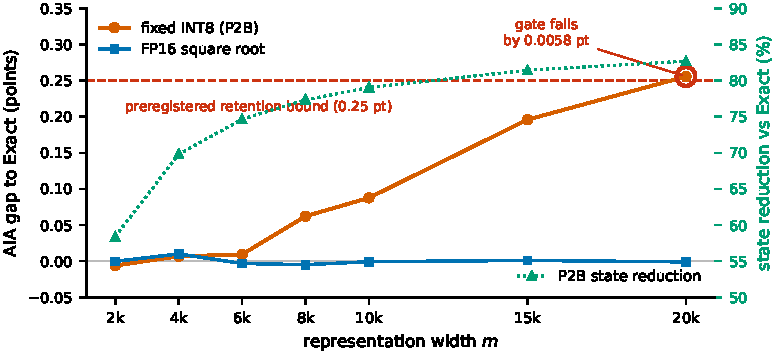
\includegraphics[width=0.86\textwidth]{fig/fig2_width_scaling.pdf}
\caption{Fixed INT8 precision does not scale with representation width.
\textbf{Left axis:} AIA gap to Exact. An FP16 square-root factor stays flat
within $0.0100$ points at every width, so the square-root update and
triangular solve are not responsible; the fixed-INT8 gap grows monotonically
beyond width $6{,}000$ and crosses the preregistered $0.25$-point retention
bound at width $20{,}000$. \textbf{Right axis:} the state reduction that
compression buys, rising from $58.4\%$ to $82.7\%$. The memory benefit and the
accuracy cost therefore grow together, which is precisely the trade-off
\S\ref{sec:adaptive} resolves. One train-only development stream.}
\label{fig:width}
\end{figure}

The gate fails at the largest width: P2B loses $0.255845$ AIA points,
exceeding the $0.25$-point limit by $0.005845$. We retain this failure rather
than relaxing the threshold, and we do not select width $15{,}000$ post hoc as
a replacement operating point. The failure lands where compression is most
valuable: state reduction grows from $58.4\%$ at width $2{,}000$ to $82.7\%$ at
$20{,}000$, because quadratic storage increasingly dominates the linear
frontend and classifier terms. Fixed INT8 therefore breaks down precisely in
the regime that motivates compressing at all.

The failure is informative because of what does \emph{not} fail alongside it.
An FP16 square-root factor stays within $0.0100$ AIA points of Exact at every
width, and the maximum solver relative residual over the whole sweep is
$5.83\times10^{-6}$. Square-root updating and triangular solution are therefore
numerically sound; the degradation is attributable to INT8 state approximation
specifically, and it is width dependent.

% ---------------------------------------------------------------------
\subsection{Why: local fidelity is the wrong target}
\label{sec:trajectory}

To locate the mechanism without altering the failed gate, we replay the locked
$10{,}000$ and $20{,}000$ streams and measure, after every task, the local
factor error $\|E_t\|$, a $16$-vector randomized estimate of the action of
$\Delta_t$, classifier and logit error, prediction agreement, and the margin
certificate of Eq.~\ref{eq:margin-certificate}.

\begin{figure}[t]
\centering
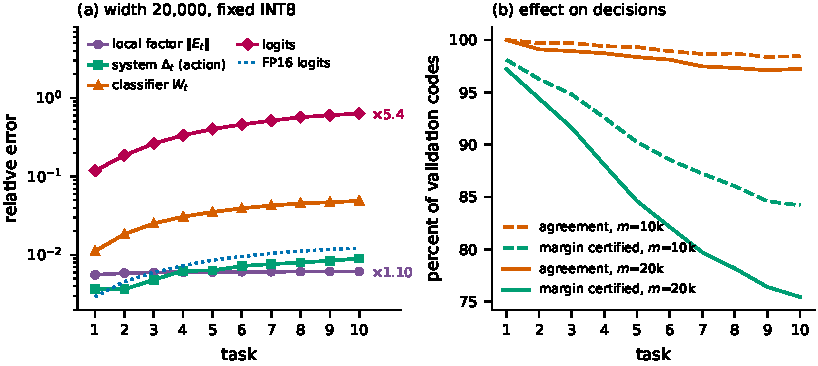
\includegraphics[width=\textwidth]{fig/fig3_error_trajectory.pdf}
\caption{Quantization error accumulates even though the quantizer does not
degrade. \textbf{(a)} Relative errors after each task at width $20{,}000$
under fixed INT8. The local factor error $\|E_t\|$ injected per task is
essentially constant ($\times1.10$ over ten tasks), while the error that
survives in the effective system, the classifier and the logits compounds
($\times5.4$ for logits). An FP16 factor shows the same compounding shape two
orders of magnitude lower, which is what
Eq.~\ref{eq:error-recurrence} predicts: accumulation is a property of the
recursion, and precision only sets its scale. \textbf{(b)} The decision-level
consequence. Prediction agreement with Exact decays slowly, but the fraction
of validation codes carrying the sufficient margin certificate of
Eq.~\ref{eq:margin-certificate} falls from $97.2\%$ to $75.4\%$ at width
$20{,}000$, and degrades faster at the larger width. One train-only
development stream; both panels are generated directly from the archived
artifact.}
\label{fig:trajectory}
\end{figure}

The decisive comparison is between the local and the accumulated quantity
(Figure~\ref{fig:trajectory}). Within a single stream at width $20{,}000$, the
local factor error injected per task is flat---it rises only $\times1.10$ from
task 1 to task 10, so the quantizer is doing the same job throughout---while
the classifier error rises $\times4.3$ and the logit error $\times5.4$. Weight
and logit error increase on every one of the nine task transitions, at both
widths. Because this comparison is made within one run, it isolates
accumulation from any change in the problem.

The same signature appears across widths. From $10{,}000$ to $20{,}000$ the
final local factor error rises by only $1.016$, yet classifier and logit errors
rise by $1.79$ and $2.00$, prediction agreement falls from $98.46\%$ to
$97.24\%$, and the margin-certified fraction falls from $84.19\%$ to $75.43\%$.
This is the pattern predicted by Eq.~\ref{eq:error-recurrence}: what grows is
not the error injected per task but the error retained across tasks, amplified
downstream through $A_t^{-1}$ as in Eq.~\ref{eq:ridge-perturbation}. FP16
behaves identically in shape while remaining two orders of magnitude smaller in
magnitude, so precision governs whether the accumulation matters, not whether
it occurs.

\paragraph{A same-byte control confirms the diagnosis.}
If local reconstruction fidelity were the binding constraint, improving it at
constant bytes should restore the gate. We test exactly that: keeping every
strict-upper value in INT8 and preserving P2B's tensor shapes and dtypes
byte-for-byte, we replace max-absolute scaling with four deterministic
alternating least-squares scale/code refinement steps, accepting a group only
when its reconstruction error does not increase. The refinement works as
intended---local factor error drops by $1.8$--$2.0\%$ after every task---and
AIA improves over P2B by $0.0368$ and $0.0057$ points at $10{,}000$ and
$20{,}000$. It nevertheless misses the retention gate at $20{,}000$ by
$0.000115$ points. We do not round the threshold. Reducing local reconstruction
MSE is therefore \emph{not} a sufficient proxy for downstream classification
error, which is the practical content of C1.

% ---------------------------------------------------------------------
\subsection{Resolution: budget-locked precision allocation}
\label{sec:adaptive}

If the constraint is accumulated rather than local error, the remedy is to
spend precision where it most reduces the error that survives. We promote
strict-upper blocks from INT8 to FP16 in decreasing order of reconstruction-MSE
reduction per added byte, subject to one fixed allowance of $25\%$ of the gap
between all-INT8 and all-FP16 payloads. Selection is label-free and uses the
factor only; the uint8 precision mask and all scale metadata are counted in
persistent state.

\begin{table}[t]
\caption{Locked six-replicate CIFAR-100 test confirmation on the controlled
RanPAC head. Mean $\pm$ sample standard deviation over six paired
class-order/projection replicates. Method, width, ridge value and precision
policy were frozen before test features were materialized; accuracy is
reported descriptively and was not a completion gate.}
\label{tab:m12}
\centering
\small
\begin{tabular}{rlrrrrr}
\toprule
Width & Backend & AIA & $A_{\mathrm{final}}$ & State (MiB) & State red. & Update/Exact\\
\midrule
$10{,}000$ & Exact    & $92.5783\pm.3829$ & $89.128\pm.075$ & $418.40$  & --      & $1.00\times$\\
$10{,}000$ & P2B      & $92.4444\pm.4135$ & $88.905\pm.135$ & $87.62$   & $79.06\%$ & $1.88\times$\\
$10{,}000$ & Adaptive & $92.5731\pm.3886$ & $89.115\pm.067$ & $98.80$   & $76.39\%$ & $2.79\times$\\
\midrule
$20{,}000$ & Exact    & $92.8220\pm.4147$ & $89.660\pm.113$ & $1{,}599.73$ & --   & $1.00\times$\\
$20{,}000$ & P2B      & $92.4956\pm.4860$ & $89.003\pm.150$ & $276.57$  & $82.71\%$ & $1.91\times$\\
$20{,}000$ & Adaptive & $92.8266\pm.4111$ & $89.678\pm.087$ & $321.28$  & $79.92\%$ & $2.91\times$\\
\bottomrule
\end{tabular}
\end{table}

Spending the budget this way removes the large-width degradation entirely
(Table~\ref{tab:m12}). Adaptive allocation changes AIA relative to Exact by
$-0.0052$ and $+0.0046$ points at the two widths, against $-0.1339$ and
$-0.3264$ for fixed P2B, so the gap diagnosed in
\S\ref{sec:scaling}--\S\ref{sec:trajectory} closes at the width where it was
largest. The small positive mean at $20{,}000$ is well inside replicate
variation and is \emph{not} an accuracy-improvement claim. Adaptive is the
higher-state, slower point on the trade-off: it spends $11$--$45$ MiB more than
P2B and $1.5\times$ its update time. The corresponding train-only development
result, and the fact that the fixed $25\%$ allowance was set before the test
split was opened, are in Appendix~\ref{app:adaptive}.

% ---------------------------------------------------------------------
\subsection{The factor structure is necessary, not incidental}
\label{sec:mechanism}

\begin{table}[t]
\caption{Train-only CIFAR mechanism ablation on one development stream. All
rows share the frontend, stream, ridge value and evaluation.}
\label{tab:mechanism}
\centering
\small
\begin{tabular}{lrrrl}
\toprule
Method & Validation AIA & $A_{\mathrm{final}}$ & State (bytes) & Outcome\\
\midrule
Exact FLY-10000                & $92.257$ & $88.140$ & $444{,}006{,}540$ & Complete\\
Direct INT8 Gram               & --       & --       & --                & \textbf{Not SPD at task 1}\\
Direct INT8 Gram + Weyl repair & $87.342$ & $80.960$ & $97{,}166{,}244$  & Complete\\
FP16 square-root               & $92.260$ & $88.130$ & $144{,}036{,}540$ & Complete\\
SRQ mixed INT8/FP32            & $92.267$ & $88.050$ & $97{,}166{,}228$  & Complete\\
\bottomrule
\end{tabular}
\end{table}

Quantizing the Gram matrix directly does not merely lose accuracy---it
destroys positive definiteness immediately, and the solve fails at task~1.
Table~\ref{tab:mechanism} uses that failure to separate the benefit of fewer
bits from the benefit of factor structure. Adding a label-free
Weyl-certified diagonal load restores a well-posed solve at essentially
identical state---the repaired Gram and SRQ differ by $16$ bytes---but costs
$4.925$ AIA points, because the certified load grows from $112.95$ to
$5{,}148.32$ times the base ridge value over ten tasks and over-regularizes the
system. Storing the same information as a factor avoids the repair entirely, by
Lemma~\ref{lem:spd}. This rules out the two tested direct-INT8 controls; it
does not prove that every conceivable direct quantizer or SPD repair is
inferior.

% ---------------------------------------------------------------------
\subsection{The backend transfers across frontends, backbones and streams}
\label{sec:portability}

\begin{table}[t]
\caption{Backend portability. Each block is an independent locked experiment.
$\Delta$AIA is the compressed backend minus Exact at the same width. Cars
values are paired means $\pm$ s.d.\ over six replicates; the CIFAR RanPAC and
GACL rows are single train-only development streams.}
\label{tab:portability}
\centering
\small
\begin{tabular}{llrrr}
\toprule
Frontend / data / backbone & Backend & AIA & $\Delta$AIA & State red.\\
\midrule
\multirow{2}{*}{RanPAC / CIFAR-100 / ViT-B/16}
 & Exact & $92.6222$ & -- & --\\
 & P2B   & $92.4608$ & $-0.1614$ & $79.06\%$\\
\midrule
\multirow{2}{*}{GACL-style / CIFAR-100 / ViT-B/16}
 & FP32 sqrt & $84.8257$ & -- & --\\
 & P2B       & $84.6869$ & $-0.1388$ & $72.64\%$\\
\midrule
\multirow{3}{*}{RanPAC / \textbf{Cars} / \textbf{ResNet-50}}
 & Exact    & $59.3517\pm.8116$ & -- & --\\
 & P2B      & $59.2855\pm.7964$ & $-0.0663\pm.0594$ & $69.70\%$\\
 & Adaptive & $59.3511\pm.8143$ & $-0.0006\pm.0076$ & $67.35\%$\\
\bottomrule
\end{tabular}
\end{table}

The backend depends on the frontend only through $\Phi_t$, so
Eqs.~\ref{eq:exact-update}--\ref{eq:qr-identity} are unchanged when the WTA
code is replaced. Table~\ref{tab:portability} tests this in three ways.

\emph{A different expansion.} On RanPAC's random-ReLU head, the independent
direct equations and our generic backend are tensor-identical after every task,
a dense FP32 square root preserves $100\%$ prediction agreement with maximum
system, weight and logit relative errors of $2.10\times10^{-6}$,
$1.24\times10^{-5}$ and $9.43\times10^{-5}$, and P2B reduces quadratic state by
$86.7\%$ for a $0.161$-point loss.

\emph{A different update regime.} GACL updates an inverse-RLS state after every
mini-batch and admits class reappearance. We adapt its recurrence to the
equivalent primal additive system; before quantization the two agree to
$99.999994\%$ of predictions, which validates the adapter independently of
compression (Appendix~\ref{app:tables}). Compressing after each of the $35$
matched mini-batches costs $0.139$ AIA points for a $72.64\%$ state reduction,
and P2B's relative logit error grows from $0.0455$ to $0.2075$ across the five
tasks---accumulation again, now at mini-batch frequency.

\emph{A different dataset and backbone.} Stanford Cars with frozen ResNet-50
changes both the data and the representation relative to the CIFAR/ViT
development line, using the published RanPAC Cars schedule and the official
split. The ridge coefficient is selected once on an $80/20$ split of the first
training task and frozen before test features exist. Adaptive tracks Exact within $0.0006$
mean AIA points at a $67.35\%$ state reduction; all $18$ units and all locked
gates pass, with maximum solver residual $8.36\times10^{-6}$ against a
preregistered $2\times10^{-5}$ limit.

These are controlled Phase-2 backend comparisons, not end-to-end reproductions:
they omit PETL and replace per-task ridge retuning with a single train-only
selected coefficient so that every backend solves the same additive system.
They establish frontend portability, not published-accuracy reproduction.

% ---------------------------------------------------------------------
\subsection{Alternatives at equal bytes, and what compression actually buys}
\label{sec:equalbudget}

\begin{figure}[t]
\centering
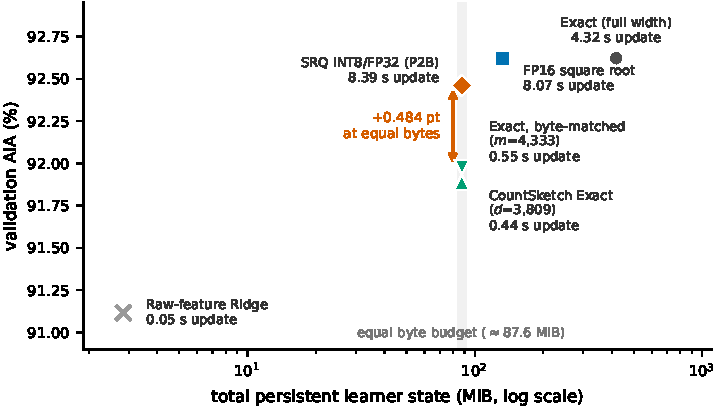
\includegraphics[width=0.86\textwidth]{fig/fig4_pareto.pdf}
\caption{Accuracy against persistent state on one train-only RanPAC stream.
The shaded column is the equal-byte comparison: the reduced Exact width and the
CountSketch dimension were derived from P2B's byte count before any accuracy
was observed. At that budget, keeping width $10{,}000$ and compressing the
factor is $0.484$ AIA points better than reducing Exact to $m=4{,}333$ and
$0.572$ better than CountSketch. Annotations give total analytic update time
over ten tasks, which is where compression costs rather than saves: P2B is
$15.3\times$ slower than byte-matched Exact. All points come from the same
stream; results from other streams are not comparable on this axis and are
reported separately.}
\label{fig:pareto}
\end{figure}

At a fixed byte budget, is compressing a wide state better than simply having a
narrower one? We derive the largest Exact width ($4{,}333$) and CountSketch
dimension ($3{,}809$) that fit inside P2B's final state from tensor shapes and
dtypes, before encoding features or observing accuracy; budget underfill is
below $0.04\%$. As Figure~\ref{fig:pareto} shows, P2B gains $0.484$ AIA points
over byte-matched Exact and $0.572$ over CountSketch, while losing $0.161$ to
full-width Exact. On the FLY
frontend the same comparison holds across three datasets: at nearly equal
state, retaining width $10{,}000$ and compressing the factor beats reducing
Exact FLY to $\approx4{,}400$--$4{,}500$ dimensions by $0.132$, $0.464$ and
$0.856$ AIA points. Against a source-pinned truncated-SVD LoRanPAC control at
matched bytes over six paired seeds, SRQ has higher mean AIA in all four
width/budget settings. That comparison retains a formal failure---its maximum
task-1 projected-solver residual is $1.91\times10^{-3}$ against a preregistered
$10^{-3}$ threshold---so we report it descriptively and trace the residual, in
Appendix~\ref{app:loranpac}, to FP32 basis non-orthogonality rather than to an
error in the ridge adapter.

\paragraph{What it costs.} Compression buys stored bytes, not runtime peak, and
the two should not be conflated. Over four paired repetitions on one Tesla T4,
persistent state falls $78.1\%$ and the serialized checkpoint $80.0\%$---the
quantities that govern checkpointing, distribution and device-resident
learners---but process-attributed whole-process peak memory falls only
$13.9\%$, because feature extraction and shared workspaces are not compressed.
The analytic stage is $1.81\times$ slower ($12.72\pm0.20$ vs $23.07\pm0.17$ s),
while total pipeline time is only $1.013\times$, since feature extraction
dominates.

% =====================================================================
\section{Limitations}
\label{sec:limitations}

\paragraph{What compression costs.}
The method is an accuracy--memory trade-off, not an accuracy improvement over
same-width Exact learning, and its analytic update is slower because it
decodes, updates by QR, re-encodes and solves after every task. The
implementation uses INT8 rather than truly packed INT4 and maintains no
error-feedback state; adding either would require counting the residual state
in the memory budget, which we have not done.

\paragraph{Scope of the evidence.}
Systems measurements use one GPU and one software stack, so the runtime-memory
and timing ratios should not be read as hardware independent. The equal-byte
controls cover reduced-width Exact, one fixed signed CountSketch, raw-feature
ridge and a truncated-SVD LoRanPAC control; learned sketches, Nystr\"om
approximations and Frequent Directions
\citep{ghashami2016,streamingridge2020} are not covered. The equal-budget and
GACL results rest on a single development seed.

\paragraph{Data provenance.}
The CIFAR-100 test split had been consumed by earlier experiments in this line,
so Table~\ref{tab:m12} is a locked confirmation rather than a first-use
benchmark; the Stanford Cars result supplies the fresh dataset and backbone. A
processed ImageNet-R split used in earlier FLY comparisons failed a
content-disjointness audit with 19 cross-split duplicate hashes, 18 of them
carrying conflicting labels, so we report it in Appendix~\ref{app:imagenetr}
with that disclosure rather than among the main results. Feature and WTA caches
contain sample-level data; they are experiment infrastructure and must never be
packaged into a deployed checkpoint or counted as evidence that the pipeline as
a whole is sample-free.

\paragraph{Unmet gates and the reach of the analysis.}
Two preregistered gates are not met, and we report both rather than adjusting
the thresholds: the width-$20{,}000$ retention bound (\S\ref{sec:scaling}) and
its same-byte refinement control (\S\ref{sec:trajectory}). The bounds in
\S\ref{sec:analysis} are worst case and conditional, and the randomized
diagnostic of \S\ref{sec:trajectory} estimates the action of $\Delta_t$ rather
than a spectral norm; neither establishes causality or measures conditioning
directly.

% =====================================================================
\section{Conclusion}

Compressing analytic continual-learning state is not the same problem as
compressing optimizer state, because the statistic accumulates and never
forgets. The binding constraint is the error retained across tasks, not the
error injected at each one: local quantization error stays flat while
classifier and logit error compound, a preregistered retention bound fails, and
a same-byte control that improves local fidelity still misses it. An exact
perturbation recurrence accounts for this, and spending a fixed precision
budget against accumulated rather than local error restores Exact accuracy to
within $0.005$ AIA points while removing roughly four fifths of the persistent
state---across three frontends, two backbones and four datasets, under gates
fixed before execution. The evidence does not establish superiority on every
metric, global Pareto optimality, or compatibility outside the fixed-feature
additive-ridge family.

% =====================================================================
\subsubsection*{Reproducibility statement}
Every experiment is specified by a versioned configuration file and produces an
archived artifact whose SHA-256 hash, source commit and preregistered gate
outcome are listed in Appendix~\ref{app:manifest}. Hyperparameter selection is
train-only throughout; the selection procedure, the authorization record
separating selection from test materialization, and the disclosed recovery
affecting one non-accuracy integrity check are described in
Appendix~\ref{app:protocol}. Proofs of Lemma~\ref{lem:spd} and
Proposition~\ref{prop:recurrence} with full assumptions are in
Appendix~\ref{app:proofs}. Anonymized code accompanies the submission.

\subsubsection*{AI use statement}
% ICLR 2027 requires this. Replace with the accurate statement before
% submission -- do not leave the placeholder.
TODO: state precisely how AI assistance was used (e.g.\ drafting, editing,
code scaffolding) and confirm the authors take full responsibility for all
content.

\bibliographystyle{iclr2027_conference}
\bibliography{references_iclr2027}

% =====================================================================
\appendix
\section{Experiment manifest, gates and artifact hashes}\label{app:manifest}
% Port from paper/EXPERIMENTS_MANIFEST.json + RESULTS_LEDGER.md.
% One row per experiment: id, artifact, SHA-256, source commit, config hash,
% preregistered gate, outcome (PASS/FAIL), test-use flag, caveat.
% NOTE (D10): ledger currently stops at M9 -- must be backfilled to M16.

\section{Protocol, selection and disclosures}\label{app:protocol}

\section{Full proofs}\label{app:proofs}

\section{Adaptive precision: development results}\label{app:adaptive}

\section{LoRanPAC equal-byte control and numerical audit}\label{app:loranpac}

\section{FLY-CL results and the ImageNet-R split disclosure}\label{app:imagenetr}

\section{Width sweep, error trajectory and per-task tables}\label{app:tables}

\end{document}
